\documentclass[11pt,a4paper,twoside]{book}
\usepackage[]{graphicx}\usepackage[]{color}
%% maxwidth is the original width if it is less than linewidth
%% otherwise use linewidth (to make sure the graphics do not exceed the margin)
\makeatletter
\def\maxwidth{ %
  \ifdim\Gin@nat@width>\linewidth
    \linewidth
  \else
    \Gin@nat@width
  \fi
}
\makeatother

\definecolor{fgcolor}{rgb}{0.345, 0.345, 0.345}
\newcommand{\hlnum}[1]{\textcolor[rgb]{0.686,0.059,0.569}{#1}}%
\newcommand{\hlstr}[1]{\textcolor[rgb]{0.192,0.494,0.8}{#1}}%
\newcommand{\hlcom}[1]{\textcolor[rgb]{0.678,0.584,0.686}{\textit{#1}}}%
\newcommand{\hlopt}[1]{\textcolor[rgb]{0,0,0}{#1}}%
\newcommand{\hlstd}[1]{\textcolor[rgb]{0.345,0.345,0.345}{#1}}%
\newcommand{\hlkwa}[1]{\textcolor[rgb]{0.161,0.373,0.58}{\textbf{#1}}}%
\newcommand{\hlkwb}[1]{\textcolor[rgb]{0.69,0.353,0.396}{#1}}%
\newcommand{\hlkwc}[1]{\textcolor[rgb]{0.333,0.667,0.333}{#1}}%
\newcommand{\hlkwd}[1]{\textcolor[rgb]{0.737,0.353,0.396}{\textbf{#1}}}%
\let\hlipl\hlkwb

\usepackage{framed}
\makeatletter
\newenvironment{kframe}{%
 \def\at@end@of@kframe{}%
 \ifinner\ifhmode%
  \def\at@end@of@kframe{\end{minipage}}%
  \begin{minipage}{\columnwidth}%
 \fi\fi%
 \def\FrameCommand##1{\hskip\@totalleftmargin \hskip-\fboxsep
 \colorbox{shadecolor}{##1}\hskip-\fboxsep
     % There is no \\@totalrightmargin, so:
     \hskip-\linewidth \hskip-\@totalleftmargin \hskip\columnwidth}%
 \MakeFramed {\advance\hsize-\width
   \@totalleftmargin\z@ \linewidth\hsize
   \@setminipage}}%
 {\par\unskip\endMakeFramed%
 \at@end@of@kframe}
\makeatother

\definecolor{shadecolor}{rgb}{.97, .97, .97}
\definecolor{messagecolor}{rgb}{0, 0, 0}
\definecolor{warningcolor}{rgb}{1, 0, 1}
\definecolor{errorcolor}{rgb}{1, 0, 0}
\newenvironment{knitrout}{}{} % an empty environment to be redefined in TeX

\usepackage{alltt}
\newcommand{\SweaveOpts}[1]{}  % do not interfere with LaTeX
\newcommand{\SweaveInput}[1]{} % because they are not real TeX commands
\newcommand{\Sexpr}[1]{}       % will only be parsed by R


% We load package by package and set package relevant parameters.
% Topics are summarized later
%%%%%%%%%%%%%%%%%%%%%%%%%%%%%%%%%%%%%%%%%%%%%%%%%%%%%%%%%%%%%%%%%%%%%%%%
% helping packages
\usepackage{ifthen}
\usepackage{calc}

\usepackage[T1]{fontenc}       % provides fonts having  accented characters 
\usepackage[latin1]{inputenc}  % allows the user to input accented characters directly from the keyboard

%%%%%%%%%%%%%%%%%%%%%%%%%%%%%%%%%%%%%%%%%%%%%%%%%%%%%%%%%%%%%%%%%%%%%%%%

\renewcommand{\baselinestretch}{1.2}
\renewcommand{\textfraction}{0}%0.2     % placement of figures
\renewcommand{\topfraction}{1}%.3
\renewcommand{\bottomfraction}{1}%.3
\renewcommand{\floatpagefraction}{1}%.3
\setcounter{bottomnumber}{3}%1

\textwidth6.3in
\textheight9.7in
\topmargin-45pt
\oddsidemargin-.15in
\evensidemargin.15in
\headsep30pt
\headheight15pt
%\footskip20pt


%%%%%%%%%%%%%%%%%%%%%%%%%%%%%%%%%%%%%%%%%%%%%%%%%%%%%%%%%%%%%%%%%%%%%%%%

\usepackage[dvipsnames]{xcolor}
\definecolor{fgcolor}{rgb}{0.345, 0.345, 0.345}
\definecolor{shadecolor}{rgb}{.97, .97, .97}
\definecolor{messagecolor}{rgb}{0, 0, 0}
\definecolor{warningcolor}{rgb}{1, 0, 1}
\definecolor{errorcolor}{rgb}{1, 0, 0}
\definecolor{DarkBlue}{rgb}{0,0,0.5451}
\definecolor{DarkGreen}{rgb}{0,0.39216,0}
\definecolor{LightYellow}{rgb}{1,1,.8}
\definecolor{orange}{rgb}{.9,0.3445,0}



%%%%%%%%%%%%%%%%%%%%%%%%%%%%%%%%%%%%%%%%%%%%%%%%%%%%%%%%%%%%%%%%%%%%%%%%
\usepackage{afterpage}
\usepackage{natbib}
\usepackage{upquote}

\usepackage[english]{babel}

%%%%%%%%%%%%%%%%%%%%%%%%%%%%%%%%%%%%%%%%%%%%%%%%%%%%%%%%%%%%%%%%%%%%%%%%%%%%%%%
%% maxwidth is the original width if it is less than linewidth
%% otherwise use linewidth (to make sure the graphics do not exceed the margin)
\makeatletter
\def\maxwidth{ %
  \ifdim\Gin@nat@width>\linewidth
    \linewidth
  \else
    \Gin@nat@width
  \fi
}
\makeatother

%%%%%%%%%%%%%%%%%%%%%%%%%%%%%%%%%%%%%%%%%%%%%%%%%%%%%%%%%%%%%%%%%%%%%%%%%%%%%%%%%%%%%%%%%%%%%%%%%%%%%%%%%%%%
% from fancyvrb
\usepackage{fancyhdr}
\usepackage{fancyvrb}
\DefineVerbatimEnvironment{Rcode}{Verbatim}{xleftmargin=2em,fontshape=sl,formatcom=\color{DarkGreen}}
\fvset{listparameters={\setlength{\topsep}{0pt}}}

%%%%%%%%%%%%%%%%%%%%%%%%%%%%%%%%%%%%%%%%%%%%%%%%%%%%%%%%%%%%%%%%%%%%%%%%%%%%%%%%%%%%%%%%%%%%%%%%%%%%%%%%%%%%%
\usepackage{float}
\usepackage{graphicx}
\usepackage[margin=2em,labelfont=bf]{caption}


%%%%%%%%%%%%%%%%%%%%%%%%%%%%%%%%%%%%%%%%%%%%%%%%%%%%%%%%%%%%%%%%%%%%%%%%
\usepackage[pdftex,plainpages=false,pdfpagelabels,pagebackref=true,colorlinks=true,pdfpagemode=UseOutlines]{hyperref}


%%%%%%%%
\usepackage{tabularx}
%%%%%%%%

%%%%%%%%%%%%%%%%%%%%%%%%%%%%%%%%%%%%%%%%%%%%%%%%%%%%%%%%%%%%%%%%%%%%%%%%
% now math stuff and other details...
\usepackage{amsmath,amsthm,amssymb}

\newtheorem{pro}{Property}[chapter]
\theoremstyle{definition}
\newtheorem{des}{Definition}[chapter]
\newtheorem{bsp}{Example}[chapter]
\newtheorem{rem}{Remark}[chapter]

\newcommand*\widebar[1]{%
  \vbox{%
    \hrule height 0.5pt%     % Line above with certain width
    \kern0.5ex%             % Distance between line and content
    \hbox{%
      \kern-0.1em%           % Distance between content and left side of box, negative values for lines shorter than content
      \ifmmode#1\else\ensuremath{#1}\fi%  % The content, typeset in dependence of mode
      \kern-0.1em%      % Distance between content and left side of box, negative values for lines shorter than content
    }% end of hbox
  }% end of vbox
}
\def\ds{\displaystyle}

\newcommand{\rr}[1]{{\ttfamily\slshape\color{DarkGreen} #1}}

\makeatletter


% clever trick to circumvent potential redefines after loading packages:
% \providecommand{\something}{}  % if it does not exist, it creates it.
%      has same syntax as \newcommand
% \renewcommand{\something}{....}
% TUGboat 29(2)


\makeatletter
%umdefinierung exisitierender befehle
\let\oldH\H
\let\oldL\L
\let\oldO\H
\let\oldS\S
\let\olda\a
\let\oldb\b
\let\oldc\c
\let\oldd\d
\let\oldk\k
\let\oldv\v
\let\oldl\l
\let\oldt\t
\let\oldu\u
\let\oldIJ\IJ
\let\oldP\P
\let\P\relax
\let\oldnorm\|

%\DefineVerbatimEnvironment{CodeInput}{Verbatim}{fontshape=sl}
%\DefineVerbatimEnvironment{CodeOutput}{Verbatim}{}

% some classical environments, up-right, with chapter numbering.
\theoremstyle{definition}
\newtheorem{definition}{Definition}[chapter]
\newtheorem{example}{Example}[chapter]
\newtheorem{remark}{Remark}[chapter]
\newtheorem{theorem}{Theorem}[chapter]



\renewcommand{\|}{|\!|}         % closer norm
\newcommand{\T}{{}^{\top}}
\newcommand\code[1]{{\tt#1}}



\newcounter{algo}
\newenvironment{algorithm}{%
  \begin{list}{
      (\arabic{algo})
    }{
      \usecounter{algo}
    }%
}{
  \end{list}
}

% some text abbreviation
\newcommand{\GLS}{\text{GLS}}
\newcommand{\RR}{\text{RR}}
\newcommand{\OR}{\text{OR}}
\newcommand{\WLS}{\text{WLS}}
\newcommand{\MLE}{\text{MLE}}
\newcommand{\OLS}{\text{OLS}}
\newcommand{\MAE}{\text{MAE}}
\newcommand{\MAD}{\text{MAD}}
\newcommand{\RMSE}{\text{RMSE}}
\newcommand{\SVAR}{\text{svar}} %silvanos new commands
\newcommand{\EVAR}{\text{evar}}
\newcommand{\LMG}{\text{LMG}}
\newcommand{\Rtwo}{\text{R}^2}



\newcommand{\ii}{\text{\i}}

\newcommand{\Bin}{\cB\mathit{\!i\!n}}
\newcommand{\Beta}{\cB\mathit{\!e\!t\!a}}
\newcommand{\Pois}{\cP\mathit{\!o\!i\!s\!s\!o\!n}}
\newcommand{\Exp}{\cE\mathit{\!x\!p}}


\DeclareMathOperator*{\argmin}{argmin}
\DeclareMathOperator*{\argmax}{argmax}
\DeclareMathOperator{\diag}{diag}
\DeclareMathOperator{\diam}{diam}
\DeclareMathOperator{\card}{card}
\DeclareMathOperator{\cov}{Cov}                   
\DeclareMathOperator{\corr}{Corr}                 
\DeclareMathOperator{\var}{Var}                   
\DeclareMathOperator{\trace}{tr}                  
\DeclareMathOperator{\E}{E}                       
\DeclareMathOperator{\P}{P}                       
\DeclareMathOperator{\pred}{p}
\DeclareMathOperator{\vect}{vec}                  
\DeclareMathOperator{\vech}{vech}                 
\DeclareMathOperator{\rank}{rank}                 
\DeclareMathOperator{\e}{e}                       
%\DeclareMathOperator{\cv}{CV}                     
\DeclareMathOperator{\GCV}{GCV}                     
\DeclareMathOperator{\CV}{CV}                     
\DeclareMathOperator{\BLUP}{BLUP}                 
\DeclareMathOperator{\MSE}{MSE}                   
\DeclareMathOperator{\MS}{MS}                   
\DeclareMathOperator{\df}{df}                   
\DeclareMathOperator{\bias}{bias}                   
\DeclareMathOperator{\eig}{eig}                   
\DeclareMathOperator{\Prec}{Prec}
\DeclareMathOperator{\mode}{mode}
\renewcommand{\SS}{\text{SS}}
\renewcommand{\d}{\mathsf{\,d}}

\def\arctanh{\qopname\relax o{arctanh}}  % as in amsopn
\newcommand{\bigo}{\cO}
\newcommand{\lito}{\text{\scriptsize{$\cO$}}}
\newcommand{\cdfPhi}{\itPhi}
\newcommand{\ml}{_\text{ML}}

\newcommand*{\stack@relbin}[3][]{%
  \mathop{#3}\limits
  \toks@{#1}%
  \edef\reserved@a{\the\toks@}%
  \ifx\reserved@a\@empty\else_{#1}\fi
  \toks@{#2}%
  \edef\reserved@a{\the\toks@}%
  \ifx\reserved@a\@empty\else^{#2}\fi
  \egroup
}%
\renewcommand*{\stackrel}{\mathrel\bgroup\stack@relbin}
\newcommand*{\stackbin}{\mathbin\bgroup\stack@relbin}
\newcommand{\simiid}{\stackrel[]{\text{iid}}{\sim}}

% Kalligraphischer Schriftsatz
\newcommand{\cA}{{\cal{A}}}
\newcommand{\cB}{{\cal{B}}} 
\newcommand{\cC}{{\cal{C}}}
\newcommand{\cD}{{\cal{D}}} 
\newcommand{\cE}{{\cal{E}}}
\newcommand{\cF}{{\cal{F}}}
\newcommand{\cG}{{\cal{G}}}
\newcommand{\cH}{{\cal{H}}}
\newcommand{\cI}{{\cal{I}}}
\newcommand{\cJ}{{\cal{J}}}
\newcommand{\cK}{{\cal{K}}}
\newcommand{\cL}{{\cal{L}}}
\newcommand{\cM}{{\cal{M}}} 
\newcommand{\cN}{{\cal{N}}}
\newcommand{\cO}{{\cal{O}}} 
\newcommand{\cP}{{\cal{P}}}
\newcommand{\cQ}{{\cal{Q}}} 
\newcommand{\cR}{{\cal{R}}} 
\newcommand{\cS}{{\cal{S}}} 
\newcommand{\cT}{{\cal{T}}}
\newcommand{\cU}{{\cal{U}}}
\newcommand{\cV}{{\cal{V}}}
\newcommand{\cW}{{\cal{W}}}
\newcommand{\cX}{{\cal{X}}} 
\newcommand{\cY}{{\cal{Y}}}
\newcommand{\cZ}{{\cal{Z}}} 


\newcommand{\IA}{{\mathbb{A}}}
\newcommand{\IB}{{\mathbb{B}}}
\newcommand{\IC}{{\mathbb{C}}}
\newcommand{\ID}{{\mathbb{D}}}
\newcommand{\IE}{{\mathbb{E}}}
\newcommand{\IF}{{\mathbb{F}}}
\newcommand{\IG}{{\mathbb{G}}}
\newcommand{\IH}{{\mathbb{H}}}
\newcommand{\II}{{\mathbb{I}}}
%\newcommand{\IJ}{{\mathbb{J}}}
\newcommand{\IK}{{\mathbb{K}}}
\newcommand{\IL}{{\mathbb{L}}}
\newcommand{\IM}{{\mathbb{M}}}
\newcommand{\IN}{{\mathbb{N}}}
\newcommand{\IO}{{\mathbb{O}}}
\newcommand{\IP}{{\mathbb{P}}}
\newcommand{\IQ}{{\mathbb{Q}}}
\newcommand{\IR}{{\mathbb{R}}}
\newcommand{\IS}{{\mathbb{S}}}
\newcommand{\IT}{{\mathbb{T}}}
\newcommand{\IU}{{\mathbb{U}}}
\newcommand{\IV}{{\mathbb{V}}}
\newcommand{\IW}{{\mathbb{W}}}
\newcommand{\IX}{{\mathbb{X}}}
\newcommand{\IY}{{\mathbb{Y}}}
\newcommand{\IZ}{{\mathbb{Z}}}


% fette griechische kleinbuchstaben
\newcommand{\balpha}{{\boldsymbol{\alpha}}}
\newcommand{\bbeta}{{\boldsymbol{\beta}}}
\newcommand{\bgamma}{{\boldsymbol{\gamma}}}
\newcommand{\bdelta}{{\boldsymbol{\delta}}}
\newcommand{\blambda}{{\boldsymbol{\lambda}}}
\newcommand{\bepsilon}{{\boldsymbol{\epsilon}}}
\newcommand{\bvarepsilon}{{\boldsymbol{\varepsilon}}}
\newcommand{\bzeta}{{\boldsymbol{\zeta}}}
\newcommand{\bfeta}{{\boldsymbol{\eta}}}  %  <----- exception !
\newcommand{\btheta}{{\boldsymbol{\theta}}{}}
\newcommand{\bvartheta}{{\boldsymbol{\vartheta}}}
\newcommand{\biota}{{\boldsymbol{\iota}}}
\newcommand{\bkappa}{{\boldsymbol{\kappa}}}
\newcommand{\bmu}{{\boldsymbol{\mu}}}
\newcommand{\bnu}{{\boldsymbol{\nu}}}
\newcommand{\bxi}{{\boldsymbol{\xi}}}
\newcommand{\bpi}{{\boldsymbol{\pi}}}
\newcommand{\bvarpi}{{\boldsymbol{\varpi}}}
\newcommand{\brho}{{\boldsymbol{\rho}}}
\newcommand{\bvarrhoi}{{\boldsymbol{\varrho}}}
\newcommand{\bsigma}{{\boldsymbol{\sigma}}}
\newcommand{\bvarsigma}{{\boldsymbol{\varsigma}}}
\newcommand{\btau}{{\boldsymbol{\tau}}}
\newcommand{\bvartau}{{\boldsymbol{\vartau}}}
\newcommand{\bupsilon}{{\boldsymbol{\upsilon}}}
\newcommand{\bphi}{{\boldsymbol{\phi}}}
\newcommand{\bvarphi}{{\boldsymbol{\varphi}}}
\newcommand{\bchi}{{\boldsymbol{\chi}}}
\newcommand{\bpsi}{{\boldsymbol{\psi}}}
\newcommand{\bomega}{{\boldsymbol{\omega}}}


% fette griechische grossbuchstaben
\newcommand{\bGamma}{{\boldsymbol{\Gamma}}}
\newcommand{\bDelta}{{\boldsymbol{\Delta}}}
\newcommand{\bTheta}{{\boldsymbol{\Theta}}}
\newcommand{\bLambda}{{\boldsymbol{\Lambda}}{}}
\newcommand{\bXi}{{\boldsymbol{\Xi}}}
\newcommand{\bPi}{{\boldsymbol{\Pi}}}
\newcommand{\bSigma}{{\boldsymbol{\Sigma}}{}}
\newcommand{\bUpsilon}{{\boldsymbol{\Upsilon}}{}}
\newcommand{\bPhi}{{\boldsymbol{\Phi}}}
\newcommand{\bPsi}{{\boldsymbol{\Psi}}}
\newcommand{\bOmega}{{\boldsymbol{\Omega}}}

% italics griechische grossbuchstaben
\newcommand{\itGamma}{{\mathit{\Gamma}}}
\newcommand{\itDelta}{{\mathit{\Delta}}}
\newcommand{\itTheta}{{\mathit{\Theta}}}
\newcommand{\itLambda}{{\mathit{\Lambda}}}
\newcommand{\itXi}{{\mathit{\Xi}}}
\newcommand{\itPi}{{\mathit{\Pi}}}
\newcommand{\itSigma}{{\mathit{\Sigma}}}
\newcommand{\itUpsilon}{{\mathit{\Upsilon}}}
\newcommand{\itPhi}{{\mathit{\Phi}}}
\newcommand{\itPsi}{{\mathit{\Psi}}}
\newcommand{\itOmega}{{\mathit{\Omega}}}



\newcommand{\A}{{\mathbf{A}}}
\newcommand{\B}{{\mathbf{B}}}
\newcommand{\C}{{\mathbf{C}}}
\newcommand{\D}{{\mathbf{D}}}
\newcommand{\bfE}{{\mathbf{E}}}    % \E: expectation
\newcommand{\F}{{\mathbf{F}}}
\newcommand{\G}{{\mathbf{G}}}
\renewcommand{\H}{{\mathbf{H}}}
\newcommand{\I}{{\mathbf{I}}}
\newcommand{\J}{{\mathbf{J}}}
\newcommand{\K}{{\mathbf{K}}}
\renewcommand{\L}{{\mathbf{L}}}
\newcommand{\bfM}{{\mathbf{M}}}
\newcommand{\N}{{\mathbf{N}}}
\renewcommand{\O}{{\mathbf{O}}}
\newcommand{\bfP}{{\mathbf{P}}}  % \P : probability
\newcommand{\Q}{{\mathbf{Q}}}
\newcommand{\bfR}{{\mathbf{R}}}
\renewcommand{\S}{{\mathbf{S}}}
\newcommand{\bfT}{{\mathbf{T}}} % \T transpose
\newcommand{\U}{{\mathbf{U}}}
\newcommand{\V}{{\mathbf{V}}}
\newcommand{\W}{{\mathbf{W}}}
\newcommand{\X}{{\mathbf{X}}}
\newcommand{\Y}{{\mathbf{Y}}}
\newcommand{\Z}{{\mathbf{Z}}}


\newcommand{\0}{{\mathbf{0}}}
\newcommand{\1}{{\mathbf{1}}}
\newcommand{\2}{{\mathbf{2}}}
\newcommand{\3}{{\mathbf{3}}}
\newcommand{\4}{{\mathbf{4}}}
\newcommand{\5}{{\mathbf{5}}}
\newcommand{\6}{{\mathbf{6}}}
\newcommand{\7}{{\mathbf{7}}}
\newcommand{\8}{{\mathbf{8}}}
\newcommand{\9}{{\mathbf{9}}}

\renewcommand{\a}{{\textbf{\textit{a}}}}
\renewcommand{\b}{{\textbf{\textit{b}}}}
\renewcommand{\c}{{\textbf{\textit{c}}}}
\newcommand{\bfd}{{\textbf{\textit{d}}}}  % \d  'dx'
\newcommand{\bfe}{{\textbf{\textit{e}}}}  % \e  l'exponentiel
\newcommand{\f}{{\textbf{\textit{f}}}}
\newcommand{\g}{{\textbf{\textit{g}}}}
\newcommand{\h}{{\textbf{\textit{h}}}}
\newcommand{\bfi}{{\textbf{\textit{i}}}}%\i  complex i, sans 'dot'
\newcommand{\bfj}{{\textbf{\textit{j}}}}
\renewcommand{\l}{{\textbf{\textit{l}}}}
\renewcommand{\k}{{\textbf{\textit{k}}}}
\newcommand{\m}{{\textbf{\textit{m}}}}
\newcommand{\bfn}{{\textbf{\textit{n}}}}
\newcommand{\bfo}{{\textbf{\textit{o}}}}
\newcommand{\p}{{\textbf{\textit{p}}}}
\newcommand{\q}{{\textbf{\textit{q}}}}
\renewcommand{\r}{{\textbf{\textit{r}}}}
\newcommand{\s}{{\textbf{\textit{s}}}}
\renewcommand{\t}{{\textbf{\textit{t}}}}
\newcommand{\bfu}{{\textbf{\textit{u}}}} %\u used in references
\renewcommand{\v}{{\textbf{\textit{v}}}}
\newcommand{\w}{{\textbf{\textit{w}}}}
\newcommand{\x}{{\textbf{\textit{x}}}}
\newcommand{\y}{{\textbf{\textit{y}}}}
\newcommand{\z}{{\textbf{\textit{z}}}}




\ifcsname hlkwd\endcsname%    ... command '#1' exists ...%
\else%  ... command '#1' does not exist ...%

\def\maxwidth{ %
  \ifdim\Gin@nat@width>\linewidth
    \linewidth
  \else
    \Gin@nat@width
  \fi
}

\definecolor{fgcolor}{rgb}{0.345, 0.345, 0.345}
\newcommand{\hlnum}[1]{\textcolor[rgb]{0.686,0.059,0.569}{#1}}%
\newcommand{\hlstr}[1]{\textcolor[rgb]{0.192,0.494,0.8}{#1}}%
\newcommand{\hlcom}[1]{\textcolor[rgb]{0.678,0.584,0.686}{\textit{#1}}}%
\newcommand{\hlopt}[1]{\textcolor[rgb]{0,0,0}{#1}}%
\newcommand{\hlstd}[1]{\textcolor[rgb]{0.345,0.345,0.345}{#1}}%
\newcommand{\hlkwa}[1]{\textcolor[rgb]{0.161,0.373,0.58}{\textbf{#1}}}%
\newcommand{\hlkwb}[1]{\textcolor[rgb]{0.69,0.353,0.396}{#1}}%
\newcommand{\hlkwc}[1]{\textcolor[rgb]{0.333,0.667,0.333}{#1}}%
\newcommand{\hlkwd}[1]{\textcolor[rgb]{0.737,0.353,0.396}{\textbf{#1}}}%

\usepackage{framed}
\newenvironment{kframe}{%
 \def\at@end@of@kframe{}%
 \ifinner\ifhmode%
  \def\at@end@of@kframe{\end{minipage}}%
  \begin{minipage}{\columnwidth}%
 \fi\fi%
 \def\FrameCommand##1{\hskip\@totalleftmargin \hskip-\fboxsep
 \colorbox{shadecolor}{##1}\hskip-\fboxsep
     % There is no \\@totalrightmargin, so:
     \hskip-\linewidth \hskip-\@totalleftmargin \hskip\columnwidth}%
 \MakeFramed {\advance\hsize-\width
   \@totalleftmargin\z@ \linewidth\hsize
   \@setminipage}}%
 {\par\unskip\endMakeFramed%
 \at@end@of@kframe}
\renewenvironment{kframe}{%
 \def\at@end@of@kframe{}%
 \ifinner\ifhmode%
  \def\at@end@of@kframe{\end{minipage}}%
  \begin{minipage}{\columnwidth}%
 \fi\fi%
 \def\FrameCommand##1{\hskip\@totalleftmargin \hskip-0\fboxsep
 \colorbox{shadecolor}{##1}\hskip-0\fboxsep
     % There is no \\@totalrightmargin, so:
     \hskip-\linewidth \hskip-\@totalleftmargin \hskip\columnwidth}%
 \MakeFramed {\advance\hsize-\width
   \@totalleftmargin\z@ \linewidth\hsize
   \@setminipage}}%
 {\par\unskip\endMakeFramed%
 \at@end@of@kframe}


\definecolor{shadecolor}{rgb}{.97, .97, .97}
\definecolor{messagecolor}{rgb}{0, 0, 0}
\definecolor{warningcolor}{rgb}{1, 0, 1}
\definecolor{errorcolor}{rgb}{1, 0, 0}
%\newenvironment{knitrout}{}{} % an empty environment to be redefined in TeX
\newenvironment{knitrout}{\setlength{\topsep}{0mm}\setlength{\fboxsep}{4mm}}{} 

\usepackage{alltt}
\IfFileExists{upquote.sty}{\usepackage{upquote}}{}

  \fi%

\makeatother
   % packages, layout and standard macros



\begin{document}
% LaTeX file for Chapter 04





\chapter{Discussion and Outlook - Some extenstions}

In the following chapter some extenstions of the LMG formula in the Bayesian framework beyond the simple linear regression model are shown. The focus is on repeated measurements models. These models extend the simple linear regression be allowing intra subject correlation between repeated measures. 

The dependence within subjects can be modeled by including random effects (mixed model) or by assuming correlated errors within a subject (marginal model). Using a random intercept model or a compound symmetry matrix for the error will result in the same model for the fixed predictors. A mixed model can be extended by including a random slope per subject, allowing for less restrictive longitudinal shapes. The marginal approach can get more freedom by different specified covariance matrices of the error terms. An unstructured covariance matrix, where no restriction are imposed, allows for the most freedom. However, depending on the number of repeated measuresments and the sample size the covariance matrix can get too large to make reasonable inference about it. 


The extenstion of the LMG formula in the Bayesian framework presented in chapter is restricted to models where the conditional variance formula can easily be applied to get the explained variance of the submodel from the regression parameters of the full model. The focus is on the fixed predictors and not on the random effects. Using the conditional variance formula to get the explained variance of the fixed predictors of the submodels should be applicable in the marginal models, where only the fixed effects are modelled anyway. In the mixed model framework the conditional variance formula is applicable to models including only random intercepts and the focus lies in the explained variance of the fixed predictors. For random-slope models there are atleast some difficulties involved, if it is possible at all the get the expalined variance of the submodel. This chapter shows a  random intercept model and a repeated measurement model with an unstructured covariance matrix.  

The first example concerns a simple random intercept model with time varying predictors.  

\section{random intercept model}

Different $\Rtwo$ metrics exist for linear mixed models. The variance of a random intercept model with regression parameter $\bbeta$ can be written as

      \begin{align} 
        \var(y) = \sigma_{f}^2  + \sigma_{\alpha}^2 + \sigma_{\epsilon}^2, 
        \end{align}

where $\sigma_{f}^2 = \var(\X \bbeta) = \bbeta^\top \bSigma_{\X \X}  \bbeta$ , $\sigma_{\alpha}^2 $ is the random intercept and $\sigma_{\epsilon}^2$ is the error term. 

An $\Rtwo$ that is guaranteed to be positive can be defined as

   \begin{align} 
\Rtwo_{\text{LMM}} = \frac{\sigma_{f}^2}{\sigma_{f}^2 + \sigma_{\alpha}^2 + \sigma_{\epsilon}^2},
\end{align}

Referenz Naka, Snyder.... It is theoretical possible that the $\Rtwo_{\text{LMM}}$ decreases when adding predictors. This may be problematic for the LMG metric, because of violation of the non-negative property. This should rarely be the case with real data. The $\Rtwo$ can not decrease when adding predictor by using the conditional variance formula on the full model to calculate the $\Rtwo$ of the submodels. In the Bayesian framework we would the sample from the posterior distributions of the parameters. 

The total variance of the full can be calculated as in equation 6 or by using the samples of the random intercept for each subject directly. The same total variance is then used for one sample of the posterior. (In a repeated measure study we often have within and between subject predictors. If we use the total variance of the full model the random intercept is fitted including all predictors. If a between subject predictor is excluded (e.g. Sex) and we would fit a new random intercept model, the random intercept parameter will in addition explain the variance that was explained by the excluded predictor. In other words it means that the model with the exluded between subject predictor will explain almost as much as the model where the predictor is included when each time a new model and therefore a new random intercept term is fitted in each model. 

When using the conditional variance formula for the $\Rtwo$ of the submodels, it only takes into account the explained variance of the fixed predictors. )


In repeated measurement studies the focus is often in within subject changes. The between subject variance estimated with the random intercept term may not be so important. The more important question may be how much the fixed predictors explain compared to the within subject error, which is

   \begin{align} 
\Rtwo_{\text{repeated}} = \frac{\sigma_{f}^2}{\sigma_{f}^2  + \sigma_{\epsilon}^2},
\end{align}

The square root of this term is known under the name correlation within subjects by ref(bland Altman 1995). Although in the paper the subject term is fitted as a factor. If we are interested in the within subject effects we can use the model including only the between subject predictor as the null model.

The following example shows a simple random intercept model with time-varying predictors. The main question is which within subject predictors are the most important ones. The between subject variance is of lower importance. 

The data are simulated from the following regression setting with $m = 4$ timepoints,

\begin{align} 
&Y_{i,j} \sim \mathcal{N}(\beta_{0}+x_{1_{i,j}} \beta_{1}+x_{2_{i,j}} \beta_{2}+x_{3_{i,j}} \beta_{3}+x_{4_{i,j}} \beta_{4} + \alpha_{i}, \, \sigma^2), \qquad i = 1, \dots, n \qquad j = 1, \dots, m
\end{align} 

where $\beta_{1} = 1$, $\beta_{2} = 1$,  $\beta_{3} = 2$ , $\beta_{4}=2$, $\sigma^2 = 1$, $\alpha_{i} \sim \mathcal{N}(0, \sigma_{\alpha}^2)$, $\X \sim \mathcal{N}(\0, \bSigma)$.

The following R code is used to simulate the data:



\begin{knitrout}
\definecolor{shadecolor}{rgb}{0.969, 0.969, 0.969}\color{fgcolor}\begin{kframe}
\begin{alltt}
\hlstd{sub}\hlkwb{<-} \hlnum{1}\hlopt{:}\hlnum{20}
\hlstd{subi} \hlkwb{<-} \hlkwd{rnorm}\hlstd{(}\hlnum{20}\hlstd{,} \hlnum{0}\hlstd{,} \hlnum{4}\hlstd{)}
\hlstd{subi}\hlkwb{<-}\hlkwd{rep}\hlstd{(subi,} \hlnum{4}\hlstd{)}
\hlstd{t} \hlkwb{<-} \hlkwd{c}\hlstd{(}\hlnum{0}\hlstd{,} \hlnum{1}\hlstd{,} \hlnum{2}\hlstd{,}\hlnum{3}\hlstd{)}
\hlstd{t} \hlkwb{<-} \hlkwd{c}\hlstd{(}\hlkwd{rep}\hlstd{(}\hlnum{0}\hlstd{,} \hlnum{20}\hlstd{),} \hlkwd{rep}\hlstd{(}\hlnum{1}\hlstd{,}\hlnum{20}\hlstd{),} \hlkwd{rep}\hlstd{(}\hlnum{2}\hlstd{,} \hlnum{20}\hlstd{),} \hlkwd{rep}\hlstd{(}\hlnum{3}\hlstd{,}\hlnum{20}\hlstd{))}

\hlstd{mu} \hlkwb{<-} \hlkwd{rep}\hlstd{(}\hlnum{0}\hlstd{,}\hlnum{4}\hlstd{)}
\hlstd{sig} \hlkwb{<-} \hlkwd{matrix}\hlstd{(}\hlnum{0.4}\hlstd{,} \hlnum{4}\hlstd{,} \hlnum{4}\hlstd{)}
\hlkwd{diag}\hlstd{(sig)} \hlkwb{<-} \hlnum{1}
\hlstd{sig[}\hlnum{3}\hlstd{,}\hlnum{4}\hlstd{]} \hlkwb{<-} \hlnum{0.9}
\hlstd{sig[}\hlnum{4}\hlstd{,}\hlnum{3}\hlstd{]} \hlkwb{<-} \hlnum{0.9}
\hlstd{sig[}\hlnum{1}\hlstd{,}\hlnum{2}\hlstd{]} \hlkwb{<-} \hlnum{0.3}
\hlstd{sig[}\hlnum{2}\hlstd{,}\hlnum{1}\hlstd{]} \hlkwb{<-} \hlnum{0.3}


\hlstd{rawvars} \hlkwb{<-} \hlkwd{mvrnorm}\hlstd{(}\hlkwc{n}\hlstd{=}\hlnum{80}\hlstd{,} \hlkwc{mu}\hlstd{=mu,} \hlkwc{Sigma}\hlstd{=sig)}

\hlstd{x1} \hlkwb{<-} \hlstd{t}\hlopt{+}\hlstd{rawvars[,}\hlnum{1}\hlstd{]}
\hlstd{x2} \hlkwb{<-} \hlstd{t}\hlopt{+}\hlstd{rawvars[,}\hlnum{2}\hlstd{]}
\hlstd{x3} \hlkwb{<-} \hlstd{t}\hlopt{+}\hlstd{rawvars[,}\hlnum{3}\hlstd{]}
\hlstd{x4} \hlkwb{<-} \hlstd{t}\hlopt{+}\hlstd{rawvars[,}\hlnum{4}\hlstd{]}

\hlstd{b1} \hlkwb{<-} \hlstd{b2}  \hlkwb{<-}\hlnum{1}
\hlstd{b3} \hlkwb{<-} \hlstd{b4} \hlkwb{<-} \hlnum{2}

\hlstd{y}\hlkwb{<-} \hlstd{x1}\hlopt{*}\hlstd{b1} \hlopt{+}\hlstd{x2}\hlopt{*}\hlstd{b2} \hlopt{+}\hlstd{x3}\hlopt{*}\hlstd{b3}\hlopt{+}  \hlstd{x4}\hlopt{*}\hlstd{b4} \hlopt{+} \hlstd{subi}\hlopt{+} \hlkwd{rnorm}\hlstd{(}\hlnum{80}\hlstd{,} \hlnum{0}\hlstd{,} \hlnum{0.1}\hlstd{)}

\hlstd{df} \hlkwb{<-} \hlkwd{data.frame}\hlstd{(}\hlkwc{y}\hlstd{=y,} \hlkwc{x1} \hlstd{= x1,} \hlkwc{x2}\hlstd{=x2,} \hlkwc{x3} \hlstd{= x3,} \hlkwc{x4} \hlstd{= x4,} \hlkwc{sub} \hlstd{=} \hlkwd{rep}\hlstd{(sub,}\hlnum{4}\hlstd{))}

\hlstd{p} \hlkwb{<-} \hlkwd{ggplot}\hlstd{(}\hlkwc{data} \hlstd{= df,} \hlkwd{aes}\hlstd{(}\hlkwc{x} \hlstd{= t,} \hlkwc{y} \hlstd{= y,} \hlkwc{group} \hlstd{= sub))}
\hlstd{p} \hlopt{+} \hlkwd{geom_line}\hlstd{()}
\end{alltt}
\end{kframe}
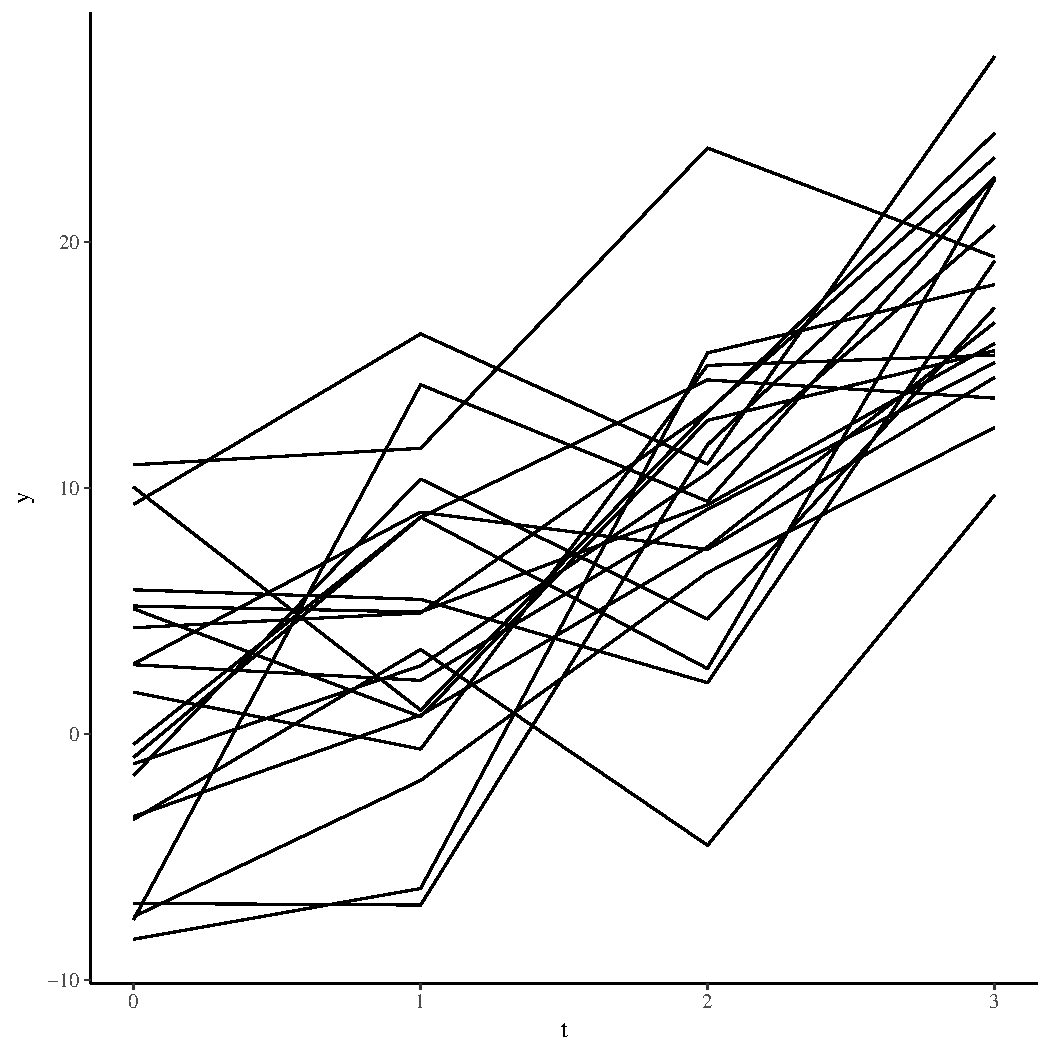
\includegraphics[width=\maxwidth]{figure/ch04_figsimdata_repeated-1} 

\end{knitrout}


The $\Rtwo$ of the submodels were first calculated according to the formula in equation ...,. The random intercept effect is not of interest. We see that most of the within subject variance is explained by the predictors. The credible intervals are very narrow. For the information about the between subject varinace we can look at the random intercept variance directly. In the second part the random intercept is included in the total variance calculation and the calculation of the $\Rtwo$ values. We see that there is a large between subject variance in this dataset. The LMG values including the between subject variance are much lower. The credible intervals are also much wider, because the uncertainty about the between subject variance is also included. In my opinion we can get more useful infromation from separating the between and within variance components when it is easy possible. Note that we assumed non stochastic predictors otherwise the credible intervals would be larger. In general it seems more reasonable to assume stochastic time-varying predictors. The variance could then be estimated by non-parameteric bootstrap, resampling whole subjects (all repeated measurements of a subject).


\begin{knitrout}
\definecolor{shadecolor}{rgb}{0.969, 0.969, 0.969}\color{fgcolor}\begin{kframe}
\begin{alltt}
\hlstd{fit} \hlkwb{<-} \hlkwd{stan_glmer}\hlstd{(y} \hlopt{~} \hlstd{x1}\hlopt{+}\hlstd{x2}\hlopt{+}\hlstd{x3}\hlopt{+}\hlstd{x4} \hlopt{+} \hlstd{(}\hlnum{1}\hlopt{|}\hlstd{sub) ,}
                                                                        \hlkwc{data} \hlstd{= df,}
                                                                        \hlkwc{chains} \hlstd{=} \hlnum{4}\hlstd{,} \hlkwc{cores} \hlstd{=} \hlnum{4}\hlstd{)}

\hlstd{post.sample} \hlkwb{<-} \hlkwd{as.matrix}\hlstd{(fit)}
\hlstd{post.sample.r} \hlkwb{<-} \hlstd{post.sample[,}\hlkwd{c}\hlstd{(}\hlnum{2}\hlopt{:}\hlnum{5}\hlstd{,(}\hlkwd{ncol}\hlstd{(post.sample)}\hlopt{-}\hlnum{1}\hlstd{)}\hlopt{:}\hlkwd{ncol}\hlstd{(post.sample))]}

\hlstd{df.rtwos} \hlkwb{<-} \hlkwd{rtwos.ri.r}\hlstd{(df[,}\hlnum{2}\hlopt{:}\hlnum{5}\hlstd{], post.sample.r)}


\hlstd{LMG.Vals}\hlkwb{<-}\hlkwd{matrix}\hlstd{(}\hlnum{0}\hlstd{,} \hlnum{4}\hlstd{,} \hlkwd{dim}\hlstd{(df.rtwos)[}\hlnum{2}\hlstd{])}

\hlkwa{for}\hlstd{(i} \hlkwa{in} \hlnum{1}\hlopt{:}\hlkwd{dim}\hlstd{(df.rtwos)[}\hlnum{2}\hlstd{])\{}

        \hlstd{gofn}\hlkwb{<-}\hlstd{df.rtwos[,i]}

        \hlstd{obj.Gelman}\hlkwb{<-}\hlkwd{partition}\hlstd{(gofn,} \hlkwc{pcan} \hlstd{=} \hlnum{4}\hlstd{,} \hlkwc{var.names} \hlstd{=} \hlkwd{names}\hlstd{(df[,}\hlnum{2}\hlopt{:}\hlnum{5}\hlstd{]))}

        \hlstd{LMG.Vals[,i]}\hlkwb{=}\hlstd{obj.Gelman}\hlopt{$}\hlstd{IJ[,}\hlnum{1}\hlstd{]}
\hlstd{\}}

\hlcom{# posterior LMG distribution of each variable}
\hlkwd{quantile}\hlstd{(LMG.Vals[}\hlnum{1}\hlstd{,],} \hlkwd{c}\hlstd{(}\hlnum{0.025}\hlstd{,} \hlnum{0.5}\hlstd{,} \hlnum{0.975}\hlstd{))}
\end{alltt}
\begin{verbatim}
##      2.5%       50%     97.5% 
## 0.1759721 0.1778704 0.1797420
\end{verbatim}
\begin{alltt}
\hlkwd{quantile}\hlstd{(LMG.Vals[}\hlnum{2}\hlstd{,],} \hlkwd{c}\hlstd{(}\hlnum{0.025}\hlstd{,} \hlnum{0.5}\hlstd{,} \hlnum{0.975}\hlstd{))}
\end{alltt}
\begin{verbatim}
##      2.5%       50%     97.5% 
## 0.1805498 0.1824204 0.1841952
\end{verbatim}
\begin{alltt}
\hlkwd{quantile}\hlstd{(LMG.Vals[}\hlnum{3}\hlstd{,],} \hlkwd{c}\hlstd{(}\hlnum{0.025}\hlstd{,} \hlnum{0.5}\hlstd{,} \hlnum{0.975}\hlstd{))}
\end{alltt}
\begin{verbatim}
##      2.5%       50%     97.5% 
## 0.3213042 0.3228832 0.3244004
\end{verbatim}
\begin{alltt}
\hlkwd{quantile}\hlstd{(LMG.Vals[}\hlnum{4}\hlstd{,],} \hlkwd{c}\hlstd{(}\hlnum{0.025}\hlstd{,} \hlnum{0.5}\hlstd{,} \hlnum{0.975}\hlstd{))}
\end{alltt}
\begin{verbatim}
##      2.5%       50%     97.5% 
## 0.3149818 0.3165701 0.3180643
\end{verbatim}
\begin{alltt}
\hlcom{# explained compared to total variance}

\hlstd{df.rtwos} \hlkwb{<-} \hlkwd{rtwos.ri.a}\hlstd{(df[,}\hlnum{2}\hlopt{:}\hlnum{5}\hlstd{], post.sample)}

\hlstd{LMG.Vals}\hlkwb{<-}\hlkwd{matrix}\hlstd{(}\hlnum{0}\hlstd{,} \hlnum{4}\hlstd{,} \hlkwd{dim}\hlstd{(df.rtwos)[}\hlnum{2}\hlstd{])}

\hlkwa{for}\hlstd{(i} \hlkwa{in} \hlnum{1}\hlopt{:}\hlkwd{dim}\hlstd{(df.rtwos)[}\hlnum{2}\hlstd{])\{}

        \hlstd{gofn}\hlkwb{<-}\hlstd{df.rtwos[,i]}

        \hlstd{obj.Gelman}\hlkwb{<-}\hlkwd{partition}\hlstd{(gofn,} \hlkwc{pcan} \hlstd{=} \hlnum{4}\hlstd{,} \hlkwc{var.names} \hlstd{=} \hlkwd{names}\hlstd{(df[,}\hlnum{2}\hlopt{:}\hlnum{5}\hlstd{]))}

        \hlstd{LMG.Vals[,i]}\hlkwb{=}\hlstd{obj.Gelman}\hlopt{$}\hlstd{IJ[,}\hlnum{1}\hlstd{]}
\hlstd{\}}

\hlcom{# posterior LMG distribution of each variable}
\hlkwd{quantile}\hlstd{(LMG.Vals[}\hlnum{1}\hlstd{,],} \hlkwd{c}\hlstd{(}\hlnum{0.025}\hlstd{,} \hlnum{0.5}\hlstd{,} \hlnum{0.975}\hlstd{))}
\end{alltt}
\begin{verbatim}
##        2.5%         50%       97.5% 
## 0.009191661 0.019669347 0.047444048
\end{verbatim}
\begin{alltt}
\hlkwd{quantile}\hlstd{(LMG.Vals[}\hlnum{2}\hlstd{,],} \hlkwd{c}\hlstd{(}\hlnum{0.025}\hlstd{,} \hlnum{0.5}\hlstd{,} \hlnum{0.975}\hlstd{))}
\end{alltt}
\begin{verbatim}
##       2.5%        50%      97.5% 
## 0.01137392 0.03076685 0.06097521
\end{verbatim}
\begin{alltt}
\hlkwd{quantile}\hlstd{(LMG.Vals[}\hlnum{3}\hlstd{,],} \hlkwd{c}\hlstd{(}\hlnum{0.025}\hlstd{,} \hlnum{0.5}\hlstd{,} \hlnum{0.975}\hlstd{))}
\end{alltt}
\begin{verbatim}
##       2.5%        50%      97.5% 
## 0.02238598 0.05498246 0.10306689
\end{verbatim}
\begin{alltt}
\hlkwd{quantile}\hlstd{(LMG.Vals[}\hlnum{4}\hlstd{,],} \hlkwd{c}\hlstd{(}\hlnum{0.025}\hlstd{,} \hlnum{0.5}\hlstd{,} \hlnum{0.975}\hlstd{))}
\end{alltt}
\begin{verbatim}
##       2.5%        50%      97.5% 
## 0.02545344 0.06020207 0.11190935
\end{verbatim}
\end{kframe}
\end{knitrout}

\section{marginal  model}

The next example concerns a repeated measurement model with an unstructured covariance error structure. The data are generated from the following model:

\begin{align} 
&Y_{i} \sim \mathcal{N}(\X_{i} \bbeta, \bSigma), \qquad i = 1, \dots, n
\end{align} 

where $\bSigma$ represents an unstructured error covariance matrix.

In the variance calculation we need to take into account that we do not have just one $\sigma^2$ parameter, but a covariance matrix $\bSigma$. The diagonal elements of $\bSigma$ represent the variance of each timepoint. The sum of the diagonal elements of $\bSigma$ represents the variance for a whole subject. When there are no missing timepoints in each subject, we can  take the mean of $\diag(\bSigma)$ to make the formula compatiable with the $\bbeta^\top \bSigma_{\X \X}  \bbeta$ of equation .... resulting in the total variance term

      \begin{align} 
        \var(\Y) = \bbeta^\top \bSigma_{\X \X}  \bbeta + \text{mean}(\diag(\bSigma)),
   \end{align}

The following R-code is used to generate the data:

\begin{knitrout}
\definecolor{shadecolor}{rgb}{0.969, 0.969, 0.969}\color{fgcolor}\begin{kframe}
\begin{alltt}
\hlstd{sub}\hlkwb{<-} \hlnum{1}\hlopt{:}\hlnum{20}
\hlstd{subi} \hlkwb{<-} \hlkwd{rnorm}\hlstd{(}\hlnum{20}\hlstd{,} \hlnum{0}\hlstd{,} \hlnum{1}\hlstd{)}
\hlstd{subi}\hlkwb{<-}\hlkwd{rep}\hlstd{(subi,} \hlnum{4}\hlstd{)}

\hlstd{mu} \hlkwb{<-} \hlkwd{rep}\hlstd{(}\hlnum{0}\hlstd{,}\hlnum{4}\hlstd{)}
\hlstd{sig} \hlkwb{<-} \hlkwd{matrix}\hlstd{(}\hlnum{0.4}\hlstd{,} \hlnum{4}\hlstd{,} \hlnum{4}\hlstd{)}
\hlkwd{diag}\hlstd{(sig)} \hlkwb{<-} \hlnum{1}
\hlstd{sig[}\hlnum{3}\hlstd{,}\hlnum{4}\hlstd{]} \hlkwb{<-} \hlnum{0.9}
\hlstd{sig[}\hlnum{4}\hlstd{,}\hlnum{3}\hlstd{]} \hlkwb{<-} \hlnum{0.9}
\hlstd{sig[}\hlnum{1}\hlstd{,}\hlnum{2}\hlstd{]} \hlkwb{<-} \hlnum{0.3}
\hlstd{sig[}\hlnum{2}\hlstd{,}\hlnum{1}\hlstd{]} \hlkwb{<-} \hlnum{0.3}

\hlstd{rawvars} \hlkwb{<-} \hlkwd{mvrnorm}\hlstd{(}\hlkwc{n}\hlstd{=}\hlnum{80}\hlstd{,} \hlkwc{mu}\hlstd{=mu,} \hlkwc{Sigma}\hlstd{=sig)}
\hlkwd{cov}\hlstd{(rawvars)}
\end{alltt}
\begin{verbatim}
##           [,1]      [,2]      [,3]      [,4]
## [1,] 0.8185433 0.1544539 0.4858672 0.4857820
## [2,] 0.1544539 0.9208422 0.2848089 0.3715627
## [3,] 0.4858672 0.2848089 1.0513613 1.0061088
## [4,] 0.4857820 0.3715627 1.0061088 1.1152070
\end{verbatim}
\begin{alltt}
\hlstd{t} \hlkwb{<-} \hlkwd{c}\hlstd{(}\hlkwd{rep}\hlstd{(}\hlnum{1}\hlstd{,} \hlnum{20}\hlstd{),}\hlkwd{rep}\hlstd{(}\hlnum{2}\hlstd{,}\hlnum{20}\hlstd{),} \hlkwd{rep}\hlstd{(}\hlnum{3}\hlstd{,} \hlnum{20}\hlstd{),} \hlkwd{rep}\hlstd{(}\hlnum{4}\hlstd{,} \hlnum{20}\hlstd{))}
\hlstd{x1} \hlkwb{<-} \hlstd{t}\hlopt{+}\hlstd{rawvars[,}\hlnum{1}\hlstd{]}
\hlstd{x2} \hlkwb{<-} \hlstd{t}\hlopt{+}\hlstd{rawvars[,}\hlnum{2}\hlstd{]}
\hlstd{x3} \hlkwb{<-} \hlstd{t}\hlopt{+}\hlstd{rawvars[,}\hlnum{3}\hlstd{]}
\hlstd{x4} \hlkwb{<-} \hlstd{t}\hlopt{+}\hlstd{rawvars[,}\hlnum{4}\hlstd{]}

\hlstd{Sig}\hlkwb{<-} \hlkwd{matrix}\hlstd{(}\hlnum{3}\hlstd{,} \hlnum{4}\hlstd{,}\hlnum{4}\hlstd{)}
\hlkwd{diag}\hlstd{(Sig)} \hlkwb{<-} \hlnum{10}
\hlstd{u} \hlkwb{<-} \hlkwd{rep}\hlstd{(}\hlnum{0}\hlstd{,} \hlnum{4}\hlstd{)}
\hlstd{Sig[}\hlnum{1}\hlstd{,}\hlnum{1}\hlstd{]} \hlkwb{<-} \hlnum{5}
\hlstd{Sig[}\hlnum{2}\hlstd{,}\hlnum{2}\hlstd{]} \hlkwb{<-} \hlnum{7}
\hlstd{Sig[}\hlnum{3}\hlstd{,}\hlnum{4}\hlstd{]} \hlkwb{<-} \hlnum{8}
\hlstd{Sig[}\hlnum{4}\hlstd{,}\hlnum{3}\hlstd{]} \hlkwb{<-} \hlnum{8}

\hlstd{Sig[}\hlnum{1}\hlstd{,}\hlnum{2}\hlstd{]} \hlkwb{<-} \hlnum{4}
\hlstd{Sig[}\hlnum{2}\hlstd{,}\hlnum{1}\hlstd{]} \hlkwb{<-}\hlnum{4}

\hlstd{Sig}
\end{alltt}
\begin{verbatim}
##      [,1] [,2] [,3] [,4]
## [1,]    5    4    3    3
## [2,]    4    7    3    3
## [3,]    3    3   10    8
## [4,]    3    3    8   10
\end{verbatim}
\begin{alltt}
\hlstd{error} \hlkwb{<-} \hlkwd{mvrnorm}\hlstd{(}\hlnum{20}\hlstd{, u, Sig)}

\hlstd{y}\hlkwb{<-} \hlstd{x1}\hlopt{*}\hlstd{b1} \hlopt{+}\hlstd{x2}\hlopt{*}\hlstd{b2} \hlopt{+} \hlstd{x3}\hlopt{*}\hlstd{b3} \hlopt{+}\hlstd{x4}\hlopt{*}\hlstd{b4} \hlopt{+}\hlkwd{c}\hlstd{(error)}


\hlstd{t} \hlkwb{<-} \hlkwd{c}\hlstd{(}\hlkwd{rep}\hlstd{(}\hlnum{1}\hlstd{,} \hlnum{20}\hlstd{),} \hlkwd{rep}\hlstd{(}\hlnum{2}\hlstd{,} \hlnum{20}\hlstd{),} \hlkwd{rep}\hlstd{(}\hlnum{3}\hlstd{,} \hlnum{20}\hlstd{),} \hlkwd{rep}\hlstd{(}\hlnum{4}\hlstd{,} \hlnum{20}\hlstd{))}
\hlstd{df} \hlkwb{<-} \hlkwd{data.frame}\hlstd{(}\hlkwc{y}\hlstd{=y,} \hlkwc{x1} \hlstd{= x1,} \hlkwc{x2}\hlstd{=x2 ,} \hlkwc{x3} \hlstd{= x3,} \hlkwc{x4} \hlstd{= x4,} \hlkwc{sub} \hlstd{=} \hlkwd{rep}\hlstd{(sub,}\hlnum{4}\hlstd{),} \hlkwc{t} \hlstd{=t)}



\hlstd{p} \hlkwb{<-} \hlkwd{ggplot}\hlstd{(}\hlkwc{data} \hlstd{= df,} \hlkwd{aes}\hlstd{(}\hlkwc{x} \hlstd{= t,} \hlkwc{y} \hlstd{= y,} \hlkwc{group} \hlstd{= sub))}
\hlstd{p} \hlopt{+} \hlkwd{geom_line}\hlstd{()}
\end{alltt}
\end{kframe}
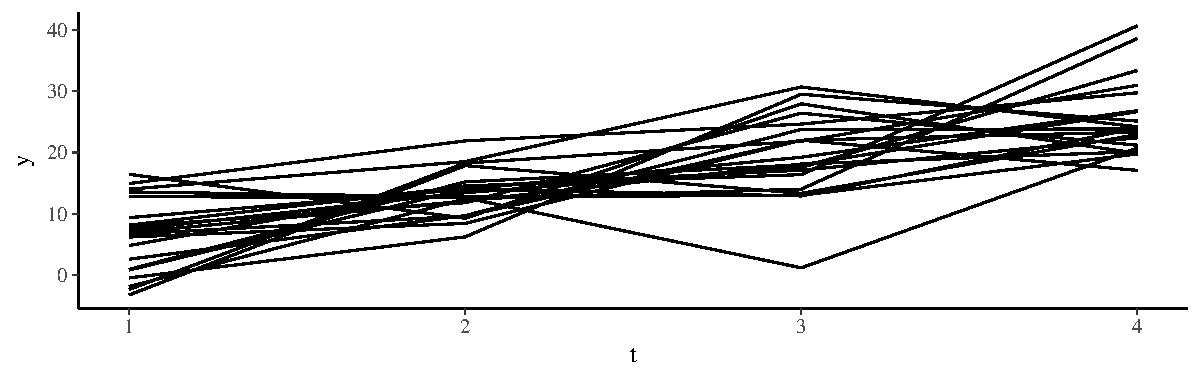
\includegraphics[width=\maxwidth]{figure/ch04_figsimdata_repeated_unstruct-1} 
\begin{kframe}\begin{alltt}
\hlcom{# Bayesian framework}

\hlstd{Y} \hlkwb{<-} \hlkwd{matrix}\hlstd{(df[,}\hlstr{'y'}\hlstd{],} \hlnum{20}\hlstd{,} \hlnum{4}\hlstd{,} \hlkwc{byrow}\hlstd{=F)}
\hlstd{x1} \hlkwb{<-} \hlkwd{matrix}\hlstd{(df[,}\hlstr{'x1'}\hlstd{],} \hlnum{20}\hlstd{,} \hlnum{4}\hlstd{,} \hlkwc{byrow}\hlstd{=F)}
\hlstd{x2} \hlkwb{<-} \hlkwd{matrix}\hlstd{(df[,}\hlstr{'x2'}\hlstd{],} \hlnum{20}\hlstd{,} \hlnum{4}\hlstd{,} \hlkwc{byrow}\hlstd{=F)}
\hlstd{x3} \hlkwb{<-} \hlkwd{matrix}\hlstd{(df[,}\hlstr{'x3'}\hlstd{],} \hlnum{20}\hlstd{,} \hlnum{4}\hlstd{,} \hlkwc{byrow}\hlstd{=F)}
\hlstd{x4} \hlkwb{<-} \hlkwd{matrix}\hlstd{(df[,}\hlstr{'x4'}\hlstd{],} \hlnum{20}\hlstd{,} \hlnum{4}\hlstd{,} \hlkwc{byrow}\hlstd{=F)}

\hlstd{N} \hlkwb{=} \hlnum{20} \hlcom{#subjects}
\hlstd{M} \hlkwb{=} \hlnum{4} \hlcom{# repeated measures}
\end{alltt}
\end{kframe}
\end{knitrout}


\begin{knitrout}
\definecolor{shadecolor}{rgb}{0.969, 0.969, 0.969}\color{fgcolor}\begin{kframe}
\begin{alltt}
\hlcom{#--------------------------------------------}

\hlstd{modelString} \hlkwb{<-} \hlstr{"model\{

# Likelihood
for(i in 1:N)\{
Y[i,1:M] ~ dmnorm(mu[i,1:M],Omega[1:M,1:M])
for(j in 1:M)\{
mu[i,j] <- beta0 + beta1*x1[i,j]+ beta2*x2[i,j]+ beta3*x3[i,j] + beta4*x4[i,j]  
\}\}

# Priors

Omega[1:M, 1:M] ~dwish(zRmat[1:M,1:M] , zRscal)
Sigma[1:M, 1:M] <- inverse(Omega)

beta0      ~ dnorm(0,0.001)
beta1      ~ dnorm(0,0.001)
beta2      ~ dnorm(0,0.001)
beta3      ~ dnorm(0,0.001)
beta4      ~ dnorm(0,0.001)

\}"}


\hlkwd{writeLines}\hlstd{( modelString ,} \hlkwc{con}\hlstd{=}\hlstr{"Jags-MultivariateNormal-model.txt"} \hlstd{)}

\hlstd{model} \hlkwb{<-} \hlkwd{jags.model}\hlstd{(}\hlkwd{textConnection}\hlstd{(modelString),}
                                                                                \hlkwc{data} \hlstd{=} \hlkwd{list}\hlstd{(}\hlkwc{Y}\hlstd{=Y,}\hlkwc{N}\hlstd{=N,}\hlkwc{M}\hlstd{=M,}\hlkwc{x1} \hlstd{= x1,} \hlkwc{x2} \hlstd{= x2,} \hlkwc{x3} \hlstd{= x3,} \hlkwc{x4} \hlstd{= x4,}     \hlkwc{zRscal} \hlstd{=} \hlkwd{ncol}\hlstd{(Y) ,}  \hlcom{# for dwish prior}
                                                                                                                                \hlkwc{zRmat} \hlstd{=} \hlkwd{diag}\hlstd{(}\hlkwc{x}\hlstd{=}\hlnum{1}\hlstd{,}\hlkwc{nrow}\hlstd{=}\hlkwd{ncol}\hlstd{(Y)) ),}
                                                                                \hlkwc{n.chains}\hlstd{=}\hlnum{3}\hlstd{)}
\end{alltt}
\begin{verbatim}
## Compiling model graph
##    Resolving undeclared variables
##    Allocating nodes
## Graph information:
##    Observed stochastic nodes: 20
##    Unobserved stochastic nodes: 6
##    Total graph size: 789
## 
## Initializing model
\end{verbatim}
\begin{alltt}
\hlstd{samp} \hlkwb{<-} \hlkwd{coda.samples}\hlstd{(model,}
                                                                                 \hlkwc{variable.names}\hlstd{=}\hlkwd{c}\hlstd{(}\hlstr{"beta1"}\hlstd{,}\hlstr{'beta2'}\hlstd{,} \hlstr{'beta3'}\hlstd{,} \hlstr{'beta4'} \hlstd{,}\hlstr{"Sigma"}\hlstd{),}
                                                                                 \hlkwc{n.iter}\hlstd{=}\hlnum{20000}\hlstd{,} \hlkwc{progress.bar}\hlstd{=}\hlstr{"none"}\hlstd{)}

\hlkwd{summary}\hlstd{(samp)}
\end{alltt}
\begin{verbatim}
## 
## Iterations = 1:20000
## Thinning interval = 1 
## Number of chains = 3 
## Sample size per chain = 20000 
## 
## 1. Empirical mean and standard deviation for each variable,
##    plus standard error of the mean:
## 
##              Mean     SD Naive SE Time-series SE
## Sigma[1,1]  5.978 2.3508 0.009597       0.013099
## Sigma[2,1]  4.576 2.3490 0.009590       0.012624
## Sigma[3,1]  2.766 2.6219 0.010704       0.011703
## Sigma[4,1]  3.512 2.4949 0.010185       0.011590
## Sigma[1,2]  4.576 2.3490 0.009590       0.012624
## Sigma[2,2]  8.095 3.2934 0.013445       0.016489
## Sigma[3,2]  1.312 3.1313 0.012783       0.013701
## Sigma[4,2]  3.566 3.2325 0.013197       0.014454
## Sigma[1,3]  2.766 2.6219 0.010704       0.011703
## Sigma[2,3]  1.312 3.1313 0.012783       0.013701
## Sigma[3,3] 12.290 5.6598 0.023106       0.025608
## Sigma[4,3]  7.791 5.3037 0.021652       0.023547
## Sigma[1,4]  3.512 2.4949 0.010185       0.011590
## Sigma[2,4]  3.566 3.2325 0.013197       0.014454
## Sigma[3,4]  7.791 5.3037 0.021652       0.023547
## Sigma[4,4]  8.247 5.9496 0.024289       0.026969
## beta1       1.223 0.2524 0.001031       0.002759
## beta2       1.031 0.2018 0.000824       0.001686
## beta3       1.283 0.5261 0.002148       0.013322
## beta4       2.411 0.5703 0.002328       0.014934
## 
## 2. Quantiles for each variable:
## 
##               2.5%     25%    50%    75%  97.5%
## Sigma[1,1]  2.9681  4.3945  5.516  7.030 11.608
## Sigma[2,1]  1.5064  3.0655  4.159  5.594 10.003
## Sigma[3,1] -0.8815  1.3080  2.474  3.891  8.056
## Sigma[4,1]  0.5801  2.1839  3.183  4.451  8.282
## Sigma[1,2]  1.5064  3.0655  4.159  5.594 10.003
## Sigma[2,2]  4.1045  5.9916  7.479  9.474 15.605
## Sigma[3,2] -3.2649 -0.1773  1.170  2.630  6.553
## Sigma[4,2]  0.1671  2.0992  3.240  4.647  8.726
## Sigma[1,3] -0.8815  1.3080  2.474  3.891  8.056
## Sigma[2,3] -3.2649 -0.1773  1.170  2.630  6.553
## Sigma[3,3]  6.3027  9.1570 11.403 14.372 23.292
## Sigma[4,3]  3.3046  5.4649  7.110  9.314 16.010
## Sigma[1,4]  0.5801  2.1839  3.183  4.451  8.282
## Sigma[2,4]  0.1671  2.0992  3.240  4.647  8.726
## Sigma[3,4]  3.3046  5.4649  7.110  9.314 16.010
## Sigma[4,4]  4.0997  6.0544  7.586  9.621 16.025
## beta1       0.7338  1.0517  1.221  1.393  1.724
## beta2       0.6451  0.8955  1.026  1.163  1.441
## beta3       0.2668  0.9337  1.278  1.628  2.326
## beta4       1.2668  2.0383  2.418  2.794  3.502
\end{verbatim}
\begin{alltt}
\hlcom{#LMG calculations}

\hlstd{samp} \hlkwb{<-} \hlkwd{coda.samples}\hlstd{(model,}
                                                                                 \hlkwc{variable.names}\hlstd{=}\hlkwd{c}\hlstd{(}\hlstr{"beta1"}\hlstd{,}\hlstr{'beta2'}\hlstd{,} \hlstr{'beta3'}\hlstd{,} \hlstr{'beta4'} \hlstd{,}\hlstr{"Sigma[1,1]"}\hlstd{,}\hlstr{"Sigma[2,2]"}\hlstd{,}\hlstr{"Sigma[3,3]"}\hlstd{,}\hlstr{"Sigma[4,4]"}\hlstd{),}
                                                                                 \hlkwc{n.iter}\hlstd{=}\hlnum{20000}\hlstd{,} \hlkwc{thin}\hlstd{=}\hlnum{20}\hlstd{,} \hlkwc{progress.bar}\hlstd{=}\hlstr{"none"}\hlstd{)}

\hlstd{post.sample} \hlkwb{<-} \hlstd{samp[[}\hlnum{1}\hlstd{]][,}\hlkwd{c}\hlstd{(}\hlnum{5}\hlopt{:}\hlnum{8}\hlstd{,} \hlnum{1}\hlopt{:}\hlnum{4}\hlstd{)]}

\hlstd{df.rtwos} \hlkwb{<-} \hlkwd{rtwos.marg}\hlstd{(df[,}\hlnum{2}\hlopt{:}\hlnum{5}\hlstd{], post.sample,} \hlnum{4}\hlstd{)} \hlcom{# 4 repeated measures}

\hlstd{LMG.Vals}\hlkwb{<-}\hlkwd{matrix}\hlstd{(}\hlnum{0}\hlstd{,} \hlnum{4}\hlstd{,} \hlkwd{dim}\hlstd{(df.rtwos)[}\hlnum{2}\hlstd{])}

\hlkwa{for}\hlstd{(i} \hlkwa{in} \hlnum{1}\hlopt{:}\hlkwd{dim}\hlstd{(df.rtwos)[}\hlnum{2}\hlstd{])\{}

        \hlstd{gofn}\hlkwb{<-}\hlstd{df.rtwos[,i]}

        \hlstd{obj.Gelman}\hlkwb{<-}\hlkwd{partition}\hlstd{(gofn,} \hlkwc{pcan} \hlstd{=} \hlnum{4}\hlstd{,} \hlkwc{var.names} \hlstd{=} \hlkwd{names}\hlstd{(df[,}\hlnum{2}\hlopt{:}\hlnum{5}\hlstd{]))}

        \hlstd{LMG.Vals[,i]}\hlkwb{=}\hlstd{obj.Gelman}\hlopt{$}\hlstd{IJ[,}\hlnum{1}\hlstd{]}
\hlstd{\}}

\hlcom{# posterior LMG distribution of each variable}
\hlkwd{quantile}\hlstd{(LMG.Vals[}\hlnum{1}\hlstd{,],} \hlkwd{c}\hlstd{(}\hlnum{0.025}\hlstd{,} \hlnum{0.5}\hlstd{,} \hlnum{0.975}\hlstd{))}
\end{alltt}
\begin{verbatim}
##      2.5%       50%     97.5% 
## 0.1077745 0.1390563 0.1671079
\end{verbatim}
\begin{alltt}
\hlkwd{quantile}\hlstd{(LMG.Vals[}\hlnum{2}\hlstd{,],} \hlkwd{c}\hlstd{(}\hlnum{0.025}\hlstd{,} \hlnum{0.5}\hlstd{,} \hlnum{0.975}\hlstd{))}
\end{alltt}
\begin{verbatim}
##       2.5%        50%      97.5% 
## 0.08137171 0.10369238 0.13062228
\end{verbatim}
\begin{alltt}
\hlkwd{quantile}\hlstd{(LMG.Vals[}\hlnum{3}\hlstd{,],} \hlkwd{c}\hlstd{(}\hlnum{0.025}\hlstd{,} \hlnum{0.5}\hlstd{,} \hlnum{0.975}\hlstd{))}
\end{alltt}
\begin{verbatim}
##      2.5%       50%     97.5% 
## 0.1450403 0.1852359 0.2153531
\end{verbatim}
\begin{alltt}
\hlkwd{quantile}\hlstd{(LMG.Vals[}\hlnum{4}\hlstd{,],} \hlkwd{c}\hlstd{(}\hlnum{0.025}\hlstd{,} \hlnum{0.5}\hlstd{,} \hlnum{0.975}\hlstd{))}
\end{alltt}
\begin{verbatim}
##      2.5%       50%     97.5% 
## 0.1522790 0.1930420 0.2260583
\end{verbatim}
\end{kframe}
\end{knitrout}







\bibliographystyle{mywiley} 
\bibliography{biblio}
\end{document}
